\documentclass{beamer}

%\usepackage[table]{xcolor}
\mode<presentation> {
  \usetheme{Boadilla}
%  \usetheme{Pittsburgh}
%\usefonttheme[2]{sans}
\renewcommand{\familydefault}{cmss}
%\usepackage{lmodern}
%\usepackage[T1]{fontenc}
%\usepackage{palatino}
%\usepackage{cmbright}
  \setbeamercovered{transparent}
\useinnertheme{rectangles}
}
%\usepackage{normalem}{ulem}
%\usepackage{colortbl, textcomp}
\setbeamercolor{normal text}{fg=black}
\setbeamercolor{structure}{fg= black}
\definecolor{trial}{cmyk}{1,0,0, 0}
\definecolor{trial2}{cmyk}{0.00,0,1, 0}
\definecolor{darkgreen}{rgb}{0,.4, 0.1}
\usepackage{array}
\beamertemplatesolidbackgroundcolor{white}  \setbeamercolor{alerted
text}{fg=red}

\setbeamertemplate{caption}[numbered]\newcounter{mylastframe}

%\usepackage{color}
\usepackage{tikz}
\usetikzlibrary{arrows}
\usepackage{colortbl}
%\usepackage[usenames, dvipsnames]{color}
%\setbeamertemplate{caption}[numbered]\newcounter{mylastframe}c
%\newcolumntype{Y}{\columncolor[cmyk]{0, 0, 1, 0}\raggedright}
%\newcolumntype{C}{\columncolor[cmyk]{1, 0, 0, 0}\raggedright}
%\newcolumntype{G}{\columncolor[rgb]{0, 1, 0}\raggedright}
%\newcolumntype{R}{\columncolor[rgb]{1, 0, 0}\raggedright}

%\begin{beamerboxesrounded}[upper=uppercol,lower=lowercol,shadow=true]{Block}
%$A = B$.
%\end{beamerboxesrounded}}
\renewcommand{\familydefault}{cmss}
%\usepackage[all]{xy}

\usepackage{tikz}
\usepackage{lipsum}

 \newenvironment{changemargin}[3]{%
 \begin{list}{}{%
 \setlength{\topsep}{0pt}%
 \setlength{\leftmargin}{#1}%
 \setlength{\rightmargin}{#2}%
 \setlength{\topmargin}{#3}%
 \setlength{\listparindent}{\parindent}%
 \setlength{\itemindent}{\parindent}%
 \setlength{\parsep}{\parskip}%
 }%
\item[]}{\end{list}}
\usetikzlibrary{arrows}
%\usepackage{palatino}
%\usepackage{eulervm}
\usecolortheme{lily}
%\usepackage[latin1]{inputenc}
\title[PS 450c] % (optional, nur bei langen Titeln nötig)
{Model Based Inference for Political Science}

\author[Grimmer]{Justin Grimmer}


\institute[Stanford University]{Professor\\
Department of Political Science\\
Stanford University}


\date{April 2nd, 2019}%[Text as Data]
%\date{\today}

\begin{document}
\begin{frame}
\titlepage
\end{frame}


\begin{frame}
\frametitle{Your Training}
\begin{itemize}
\item[0)] Math Camp
\item[1)] Pol 450A: Regression
\item[2)] Pol 450B: Design-Based Inference
\item[3)] \alert{Pol 450C: Model-Based Inference}
\item[4)] POL 450D: Topics in Quantitative Methods
\item[] $\vdots$
\end{itemize}

\end{frame}




\begin{frame}
\frametitle{Why Models?}

Design-based inference:
\begin{itemize}
\item[-] Randomness: comes from treatment assignment
\item[-] Examples: Experiments, Survey sampling, selection on observables
\item[-] Reliable, Clear, and Precise
\end{itemize}

\end{frame}



\begin{frame}
\frametitle{Why Models?}

\begin{itemize}
\item[-] Causal Inference$\leadsto$ Just One Goal! \pause
\invisible<1>{\item[-] Descriptive Inference (Measurement)} \pause
\begin{itemize}
\invisible<1-2>{\item[-] What \% of Latino voters supported Trump?} \pause
\invisible<1-3>{\item[-] Where do elected officials fall on ideological spectrum?} \pause
\invisible<1-4>{\item[-] What \% of time do Women speak in community meetings?} \pause
\invisible<1-5>{\item[-] When do diplomates discuss credibility concerns?} \pause
\end{itemize}
\invisible<1-6>{\item[-] Predictive Inference } \pause
\begin{itemize}
\invisible<1-7>{\item[-] When is war likely?} \pause
\invisible<1-8>{\item[-] Who will win the election?} \pause
\invisible<1-9>{\item[-] How long will the regime last?} \pause
\end{itemize}
\invisible<1-10>{\item[-] Exploratory Inference } \pause
\begin{itemize}
\invisible<1-11>{\item[-] What issues do women raise in community meetings?} \pause
\invisible<1-12>{\item[-] What do diplomats say in cables?} \pause
\end{itemize}
\invisible<1-13>{\item[-] Combination (heterogeneous treatment effects)} \pause
\end{itemize}
\invisible<1-14>{All require \alert{models}}



\end{frame}




\begin{frame}
\frametitle{Course Goals}

\pause
\begin{itemize}
\invisible<1>{\item[1)] Proficient \alert{user} of likelihood based methods} \pause
\invisible<1-2>{\item[2)] An {\huge introduction} to a sophisticated understanding of theoretical tools $\leadsto$ rest of your career} \pause
\invisible<1-3>{\item[3)] An introduction to numerical optimization and sophisticated estimation procedures} \pause
\invisible<1-4>{\item[4)] An introduction to basic machine learning methods } \pause
\invisible<1-5>{\item[5)] Develop applied data analysis skills} \pause
\invisible<1-6>{\item[6)] Continue improving programming skills}
\end{itemize}


\end{frame}


\begin{frame}
\frametitle{How to Accomplish those Goals?}

\begin{itemize}
\item[1)] Introduce lots of tools$\leadsto$ common logic unifying them
\item[2)] Use proofs + simulation to establish properties of estimators
\item[3)] Applied data in both problem sets and a replication assignment
\item[4)] Lots of hard work!!
\end{itemize}

\end{frame}



\begin{frame}
\frametitle{Course Logistics}

Lecture: Monday 900am-1050am GSL.   \\ \pause
\invisible<1>{TA: Matt Tyler} \pause  \\
\invisible<1-2>{Attendance Policy:} \pause \invisible<1-3>{ Grad School is your job. } \pause \invisible<1-4>{ Show up to work. } \pause \invisible<1-5>{(But you might have reasons to be absent too, which is fine just let me know so we can make sure you don't fall behind!)}

\end{frame}


\begin{frame}
Prerequisites:
\begin{itemize}
\item[1)] Math Camp
\item[2)] POL 450A
\item[3)] POL 450B
\item[OR] My permission  (if you haven't done 1-3, you shouldn't take the class)
\end{itemize}

Get some books!
\end{frame}



\begin{frame}
\frametitle{Evaluation}
Five components to evaluation:

\begin{itemize}
\item[1)] Homework (30\% ): Weekly homework assignments to develop core intuition in class.  Use {\tt R} markdown to submit
\item[2)] Midterm Exam (15\% ): \alert{May 14th} Closed Book, Pencil + Paper
\item[3)] Final Exam (25\% ): Closed Book, Computer Based
\item[4)] Replication Project (25\%): (More on next slide)
\item[5)] Participation: ask lots of questions! 
\end{itemize}


\end{frame}


\begin{frame}
\frametitle{Replication Project}

\begin{itemize}
\item[-] Team of \alert{two}: identify paper, replicate, and extend results \pause
\invisible<1>{\item[-] Science only proceeds if we know the strength of our findings.  Procedural objections are almost never made in good faith (but you should be polite + nice to people)} \pause
\invisible<1-2>{\item[-] Scholars worked really hard on project, you'll learn a lot from them} \pause
\invisible<1-3>{\item[-] Please talk to Matt and me about project selection$\leadsto$ must be quantitative data} \pause
\invisible<1-4>{\item[-] Discuss communication with authors with me before writing them} \pause
\invisible<1-5>{\item[-] Focus on \alert{substance} } \pause
\end{itemize}
\invisible<1-6>{Timeline} \pause

\begin{itemize}
\invisible<1-7>{\item[-] 4/18: Discuss paper select + project with Brad and me } \pause
\invisible<1-8>{\item[-] 5/16: Confirm replication of original results} \pause
\invisible<1-9>{\item[-] 5/30: \alert{20 page maximum} replication and extension due} \pause
\begin{itemize}
\invisible<1-10>{\item[-] \LaTeX document pdf} \pause
\invisible<1-11>{\item[-] Includes references, figures, tables, etc} \pause
\invisible<1-12>{\item[-] \alert{Replication code}} \pause
\end{itemize}
\end{itemize}


\end{frame}


\begin{frame}

\huge

Probability

\end{frame}



\begin{frame}


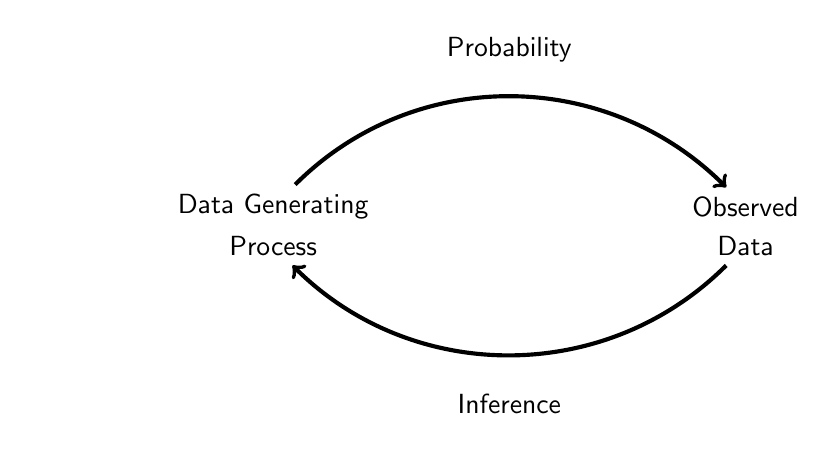
\begin{tikzpicture}
\node (dum) at (-8, 8) [] {} ;
\node (dgp) at (-5, 8) [] {Data Generating} ;
\node (dgp2) at (-5, 7.5) [] {Process} ;

\node (obs) at (1, 8) [] {Observed} ;
\node (obs2) at (1, 7.5) [] {Data} ;


\invisible<1>{\draw[->, line width = 1.5 pt] (dgp) to [out = 45, in = 135] (obs)  ; }
\invisible<1-2>{\draw[->, line width = 1.5 pt] (obs2) to [out = 225, in = 315] (dgp2); }


\invisible<1>{\node (prob) at (-2, 10) [] {Probability} ; }

\invisible<1-2>{\node (inference) at (-2, 5.5) [] {Inference} ;  }



\end{tikzpicture}


\pause \pause


\end{frame}


\begin{frame}
\frametitle{Probability Theory $\leadsto$ Refresher}

\begin{itemize}
\item[1)] Model of Probability, Axioms of Probability Function
\item[2)] Definition of Random Variable
\item[3)] Univariate ideas: Expectation, Variance
\item[4)] Multivariate ideas: Joint Distribution, Independence
\end{itemize}

We will review many random variables + properties as we develop data generating processes


\end{frame}



\begin{frame}
\frametitle{Model of Probability}

\pause

\begin{itemize}
\invisible<1>{\item[1)] Sample Space: set of all things that can occur} \pause
\invisible<1-2>{\item[2)] Events: subsets of the sample space} \pause
\invisible<1-3>{\item[3)] Probability: chance of an event} \pause
\begin{itemize}
\invisible<1-4>{\item[a)] For all events $E$} \pause
\begin{eqnarray}
\invisible<1-5>{0 & \leq & P(E) \leq 1 \nonumber } \pause
\end{eqnarray}
\invisible<1-6>{\item[b)]  P(Sample Space) = 1} \pause
\invisible<1-7>{\item[c)] For all sequences of mutually exclusive events (they share no outcomes) $E_{1}, E_{2}, \hdots, E_{N}$ (where $N \rightarrow \infty$ )} \pause
\begin{eqnarray}
\invisible<1-8>{P(\cup_{i=1}^{N} E_{i}) &= & \sum_{i=1}^{N} P(E_{i} ) \nonumber } \pause
\end{eqnarray}

\end{itemize}


\end{itemize}


\end{frame}


\begin{frame}
\frametitle{Random Variable}


A Random Variable $X$ is a function from the sample space to \alert{real numbers}.  In notation:
\begin{eqnarray}
X & : & \text{Sample Space} \rightarrow \Re \nonumber
\end{eqnarray}

\pause


\begin{itemize}
\invisible<1>{\item[-] $X$'s domain are all outcomes (Sample Space)} \pause
\invisible<1-2>{\item[-] $X$'s range is the Real line (or subset of it)} \pause
\invisible<1-3>{\item[-] If $X$ is defined on outcomes that are discrete, we can write a probability mass function: } \pause
\begin{eqnarray}
\invisible<1-4>{p(x) & = &  P(X = x)  \nonumber } \pause
\end{eqnarray}
\invisible<1-5>{\item[-] If $X$ is defined on outcomes that are continuous, we can write a probability density function, $f(x)$:} \pause
\begin{eqnarray}
\invisible<1-6>{P(X \in [a, b]) & = & \int_{a}^{b} f(x) dx \nonumber } \pause
\end{eqnarray}
\invisible<1-7>{For all $[a,b] \in \Re$} \pause
\end{itemize}

\end{frame}


\begin{frame}
\frametitle{Expectation}

Suppose $X$ is a random variable, then: \pause
\begin{itemize}
\invisible<1>{\item[-] $E[X] = \sum_{x: p(x)>0} x p(x) $ if $X$ is discrete}\pause
\invisible<1-2>{\item[-] $E[X] = \int_{-\infty}^{\infty } x f(x) dx $ is continuous}\pause
\end{itemize}
\invisible<1-3>{Suppose $g:\Re \rightarrow \Re$, then }\pause
\begin{itemize}
\invisible<1-4>{\item[-] $E[g(X)] = \sum_{x: p(x)>0} g(x) p(x) $ (discrete)}\pause
\invisible<1-5>{\item[-] $E[g(X)] = \int_{-\infty}^{\infty} g(x) f(x) dx$ (continuous )}\pause
\end{itemize}
\invisible<1-6>{Variance of $X$ is }\pause
\begin{eqnarray}
\invisible<1-7>{\text{Var}(X) & = & E[ ( X - E[X] )^{2}] \nonumber \\}\pause
\invisible<1-8>{			  & = & E[X^2] - 2 E[ X E[X]] + E[X]^{2} \nonumber \\}\pause
\invisible<1-9>{			  & = & E[X^2] - E[X]^2\nonumber}
\end{eqnarray}


\end{frame}



\begin{frame}

\huge

Random variables $\leadsto$ Build Model

\end{frame}



\begin{frame}
\frametitle{Participation}

Model individual $i$'s voter turnout decision, $Y$ \pause  \\

\begin{eqnarray}
\invisible<1>{Y & = & 1 \text{, $i$ turns out to vote} \nonumber} \pause  \\
\invisible<1-2>{Y & = & 0 \text{, $i$ does not vote} \nonumber} \pause  \\
\invisible<1-3>{P(Y = 1) & = & \pi \nonumber } \pause
\end{eqnarray}

\invisible<1-4>{$Y \sim \text{Bernoulli} (\pi)$}

\end{frame}



\begin{frame}
\frametitle{Participation}


$Y$ is a Bernoulli Random Variable\\

PMF:
\begin{eqnarray}
P(Y = y) = p(y) &= & \pi^{y} (1- \pi)^{1-y} \nonumber
\end{eqnarray}

for $y \in \{0, 1\}$ (0 otherwise)\\


\pause
\begin{eqnarray}
\invisible<1>{E[Y] & = & 1 \times P(Y = 1) + 0 \times P(Y = 0) \nonumber \\} \pause
	\invisible<1-2>{& = & \pi  + 0 (1- \pi)  = \pi \nonumber \\} \pause
\invisible<1-3>{\text{var}(Y) & = & E[Y^{2} ] - E[Y]^{2} \nonumber \\} \pause
\invisible<1-4>{E[Y^{2}] & = & 1^2 P(Y = 1)  + 0^{2} P(Y = 0 ) \nonumber \\} \pause
	\invisible<1-5>{& = & P(Y = 1) = \pi \nonumber \\} \pause
\invisible<1-6>{\text{var}(Y) & = & \pi  - \pi^{2} 		\nonumber \\} \pause
\invisible<1-7>{& = & \pi (1 - \pi ) \nonumber }
\end{eqnarray}

\end{frame}


\begin{frame}
\frametitle{Joint Random Variables: Many Turnout Decisions}

\begin{itemize}
\item[-] Interested in many individual's turnout decisions $(i = 1, \hdots, N)$
\item[-] Model joint decisions $\boldsymbol{Y} = (Y_{1}, Y_{2}, \hdots, Y_{N})$
\end{itemize}


Define:
\begin{eqnarray}
p(Y_{1} = y_{1}, Y_{2} = y_{2}, \hdots, Y_{N} = y_{N} ) & = & p(\boldsymbol{y}) \nonumber
\end{eqnarray}

This is \alert{very} complicated $\leadsto$ Let's simplify


\end{frame}


\begin{frame}
\frametitle{Joint Random Variables: Many Turnout Decisions}
Independent Random Variables: \\
Random variables $Y_{1}, Y_{2}, \hdots, Y_{N}$ are independent if \pause
\begin{eqnarray}
\invisible<1>{P(Y_{1} = y_{1}, Y_{2} = y_{2} , \hdots, Y_{N} = y_{N})  & =  &  \nonumber \\} \pause
\invisible<1-2>{P(Y_{1} = y_{1})P( Y_{2} = y_{2}) \hdots P(Y_{N} = y_{N}) & = & \nonumber \\} \pause
\invisible<1-3>{\prod_{i=1}^{N} P(Y_{i} = y_{i}) \nonumber } \pause
\end{eqnarray}


\invisible<1-4>{$Y_{i} \sim \text{Bernoulli} (\pi) $ \\} \pause
\invisible<1-5>{\alert{I}ndependent, \alert{I}dentically, \alert{D}istributed (IID)\\} \pause
\invisible<1-6>{\alert{Assumption}$\leadsto$ similar to what assumption from design-based inference?}


\end{frame}


\begin{frame}
\frametitle{Joint Random Variables: Many Turnout Decisions}
Suppose $Y_{i} \sim \text{Bernoulli}(\pi)$

\begin{eqnarray}
p(\boldsymbol{y}) & = & \prod_{i=1}^{N} P(Y_{i} = y_{i})\nonumber \\
				  & = & \prod_{i=1}^{N} \pi^{y_{i} } (1- \pi)^{1- y_{i} } \nonumber \\
				  & = & \pi^{\sum_{i=1}^{N} y_{i} } (1 - \pi)^{N - \sum_{i=1}^{N} y_{i}} \nonumber
\end{eqnarray}




\end{frame}




\begin{frame}
\frametitle{Joint Random Variables: Many Turnout Decisions}
Suppose $Y_{i} \sim \text{Bernoulli}(\pi_{\alert{i}})$ \\
\alert{Independent}

\begin{eqnarray}
p(\boldsymbol{y}) & = & \prod_{i=1}^{N} P(Y_{i} = y_{i})\nonumber \\
				  & = & \prod_{i=1}^{N} \pi_{i} ^{y_{i} } (1- \pi_{i} )^{1- y_{i} } \nonumber
\end{eqnarray}


Key insight:
\begin{itemize}
\item[-] Given $\pi_{i} \leadsto$ probability of $\boldsymbol{y}$ \\
\item[-] Given $\boldsymbol{y}$ we should be able to learn something about $\pi_{i}$
\end{itemize}

\end{frame}

\begin{frame}
\frametitle{Modeling Incumbent Vote Share}


Suppose we are interested in modeling an incumbent's vote share $Y_{i}$.\\
Assume that $Y_{i}$ is a \alert{Normal} random variable.  Specifically, we will assume:

\begin{eqnarray}
Y_{i} & \sim &  \text{Normal}(\mu, \sigma^{2}) \nonumber
\end{eqnarray}

Equivalently, a normal random variable has \alert{pdf}:


\begin{eqnarray}
f(y) & = & \frac{1}{\sqrt{2 \pi \sigma^2}  } \exp\left( \frac{ - (y - \mu )^ 2 }{2\sigma^2}\right)\nonumber
\end{eqnarray}


Properties of normal random variables:
\begin{itemize}
\item[-] $E[Y_{i}] =  \mu $
\item[-] $\text{var}(Y_{i}) = \sigma^2$
\end{itemize}


\end{frame}


\begin{frame}
\frametitle{Modeling Many Incumbents' Vote Share}


Suppose we are interested in many Congressional incumbents' vote shares\\
Assume $Y_{i} \sim \text{Normal}(\mu_{i}, \sigma^2)$\\
independent (non-identical) samples $\leadsto \boldsymbol{Y} $\\

\begin{eqnarray}
f(\boldsymbol{y} ) & = & \prod_{i=1}^{N} f(y_{i} ) \nonumber\\
					& = & \prod_{i=1}^{N}\frac{1}{\sqrt{2 \pi \sigma^2}  } \exp\left( \frac{ - (y_{i} - \mu_{i} )^ 2 }{2\sigma^2}\right)\nonumber \\
					& = & \frac{1}{ \left( 2 \pi \sigma^2  \right)^{N/2}} \exp \left(\sum_{i=1}^{N} \frac{- (y_i - \mu_{i} )^2}{2\sigma^2}   \right) \nonumber
\end{eqnarray}


How do we make inferences using the model?

\end{frame}

\begin{frame}
\frametitle{Modeling Many Incumbents' Vote Share}

Define $\boldsymbol{\mu} = (\mu_{1}, \mu_{2}, \hdots, \mu_{N})$


\begin{eqnarray}
f(\boldsymbol{y}, \underbrace{\boldsymbol{\mu}, \sigma^2}_{parameters}) & = & \frac{1}{ \left( 2 \pi \sigma^2  \right)^{N/2}} \exp \left(\sum_{i=1}^{N} \frac{- (y_i - \mu_{i} )^2}{2\sigma^2}   \right) \nonumber
\end{eqnarray}

Writing down model of $\boldsymbol{y}$ creates link between data, parameters\\
All inferences depend \alert{initial modeling assumption} (that won't be reflected in other measures of uncertainty)

\end{frame}


\begin{frame}
\frametitle{Probability Term Refresher}

\pause
\begin{itemize}
\invisible<1>{\item[1)] CDF} \pause
\invisible<1-2>{\item[2)] Marginal distribution, conditional density} \pause
\invisible<1-3>{\item[3)] Scale/Location (Normal distribution is a ...)} \pause
\invisible<1-4>{\item[4)] $X$ is a random variable, $a$ and $b$ are constants.  $E[aX + b]$, $\text{var}[aX + b]$} \pause
\invisible<1-5>{\item[5)] Bayes' Rule}
\end{itemize}



\end{frame}


\begin{frame}
Wednesday: Introduction to Likelihood Theory of Inference (inversion)\\



\end{frame}



\end{document}
